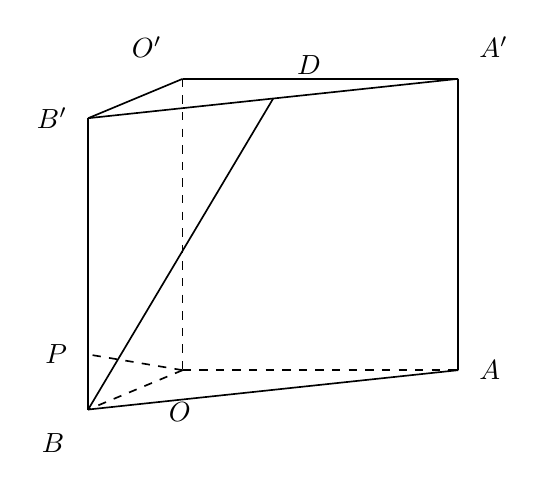
\begin{tikzpicture}[line width=.6pt, font=\normalsize]
\coordinate (O) at (1.5,0.5);
\coordinate (A) at (5,0.5);
\coordinate (B) at (0.3,0);
\coordinate (Oprime) at (1.5,4.2);
\coordinate (Aprime) at (5,4.2);
\coordinate (Bprime) at (0.3000000000,3.7000000000);
\coordinate (D) at (2.6500000000,3.9500000000);
\coordinate (P) at (0.3,0.7);
% top triangle O'A'B'
\draw (Oprime) -- (Aprime);
\draw (Oprime) -- (Bprime);
\draw (Bprime) -- (D) -- (Aprime);
% bottom triangle OAB
\draw (A) -- (B);
\draw[dashed] (O) -- (A);
\draw[dashed] (O) -- (B);
% lateral edges
\draw (Aprime) -- (A);
\draw (B) -- (Bprime);
\draw[dashed] (Oprime) -- (O);
% interior segment B-D
\draw (B) -- (D);
% OP segment, P on BB'
\draw[dashed] (O) -- (P);
% labels with clearance
\node[above left=4pt] at (Oprime) {$O'$};
\node[above right=4pt] at (Aprime) {$A'$};
\node[left=4pt] at (Bprime) {$B'$};
\node[above right=5pt,xshift=0pt,yshift=0pt] at (D) {$D$};
\node[below left=5pt] at (B) {$B$};
\node[right=4pt] at (A) {$A$};
\node[below=5pt,xshift=-1pt,yshift=-3pt] at (O) {$O$};
\node[left=4pt] at (P) {$P$};
\end{tikzpicture}
